\section{Results}
\label{sec:results}

\subsection{Wrappers hide answers the model knows}
\label{sec:lost}

Adding one neutral sentence to the plain prompt loses \FloorLost{} of known answers, depending on the model. This noise floor is measured on the short plain prompt; plain prose is the control of the same length. Wrappers lose many more answers (Figure~\ref{fig:behaviour}). Averaged over the three lengths:
\begin{itemize}
\item tool results, web pages and email threads lose \LostStruct{} of known answers, depending on the model;
\item plain prose loses \LostProse{};
\item server logs lose \LostLog{}, and up to \LostLogMax{} at one length.
\end{itemize}
On average, the interface formats hide about as many answers as plain prose of the same length, so the loss does not need markup. Logs are the exception: they are the most damaging wrapper for \LogWorstModels{}, while \LogMildModels{} \LogMildVerb{} at most five points more to logs than to any other wrapper. Length has no consistent effect: in the models hurt most by logs, logs lose most at the middle length, and the other wrappers change by a few points from one length to the next.

\begin{figure*}[t]
\centering
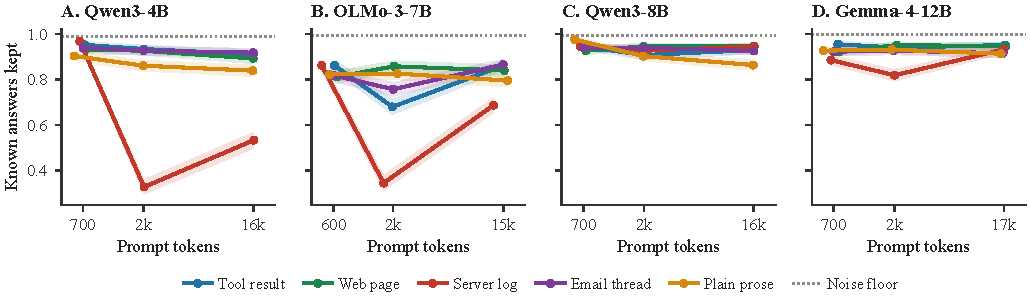
\includegraphics[width=\textwidth]{fig_behaviour.pdf}
\caption{\textbf{Known answers kept inside wrappers.} Share of known test items whose reply still contains the known answer, for each wrapper and prompt length (log scale; lengths differ slightly between tokenizers). The dotted line is the noise floor: the share kept when one neutral sentence is added to the plain prompt. Bands are 95\% intervals.}
\label{fig:behaviour}
\end{figure*}

How much wrapper sits between the question and the closing instruction matters for logs. For Qwen3-4B we also ran every wrapper with about 64 instead of about 512 tokens of wrapper after the question. Logs then lost \LostLogShortTail{} of known answers instead of \LostLogLongTail{}. The other four wrappers, averaged, lost \LostOtherShortTail{} in both layouts (Appendix~\ref{app:tail}).

\subsection{What replaces a lost answer}
\label{sec:types}

We sorted every lost answer into one of three kinds by the first line of the reply (Appendix~\ref{app:types} gives the rules):
\begin{itemize}
\item \emph{about the wrapper}: the reply describes the wrapper's content, such as ``The logs show that multiple jobs are failing'';
\item \emph{not there}: the reply says the answer cannot be given, such as ``The provided text does not contain information about the headquarters location of Taito Corporation'';
\item \emph{wrong answer}: the reply gives another answer, such as ``Sydney'' for the capital of Australia.
\end{itemize}
Table~\ref{tab:types} shows the result over all four models. Logs change the task: \TypeLogTask{} of the answers they hide are replaced by a description of the log. The other wrappers rarely do this. Their lost answers become wrong answers or claims that the text holds no answer. Plain prose draws such claims most often (\TypeProseScope{} of its losses), although every question asks for general knowledge that no text needs to supply.

\begin{table}[t]
\centering
\footnotesize
\setlength{\tabcolsep}{4pt}
\begin{tabular}{@{}lcccr@{}}
\toprule
Wrapper & About the & Not & Wrong & $n$ \\
 & wrapper & there & answer & \\
\midrule
Tool result & 2\% & 21\% & 77\% & 980 \\
Web page & 3\% & 49\% & 48\% & 923 \\
Server log & 64\% & 8\% & 28\% & 2{,}344 \\
Email thread & 1\% & 46\% & 53\% & 1{,}010 \\
Plain prose & 0\% & 73\% & 27\% & 1{,}207 \\
\bottomrule
\end{tabular}

\caption{\textbf{What replaces the lost answers}, as a share of all lost answers for each wrapper, over the four models and three lengths. $n$ is the number of lost answers.}
\label{tab:types}
\end{table}

\begin{figure*}[t]
\centering
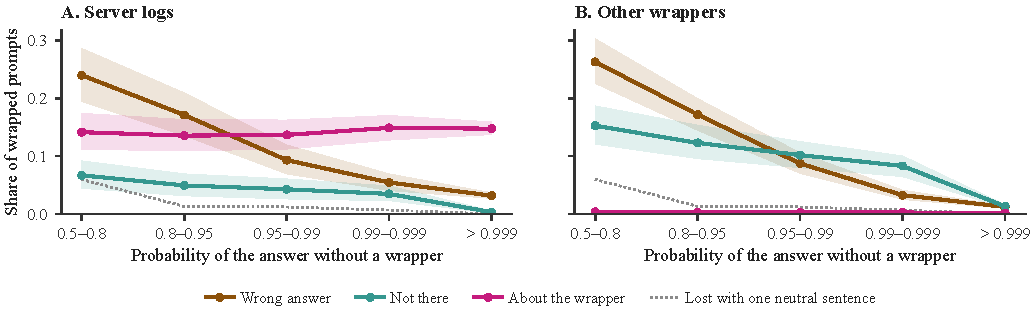
\includegraphics[width=\textwidth]{fig_confidence.pdf}
\caption{\textbf{What wrapped prompts produce, by how sure the model is of the answer without a wrapper.} Known test items are grouped by the probability each model gives the full answer in the plain prompt (\BinN{} wrapped prompts per group, over all four models, wrappers and lengths). Each coloured line is the share of wrapped prompts that lose the answer in one way; the remaining prompts keep it. The dotted line is the share lost when one neutral sentence is added instead. Bands are 95\% intervals.}
\label{fig:confidence}
\end{figure*}

\begin{figure*}[t]
\centering
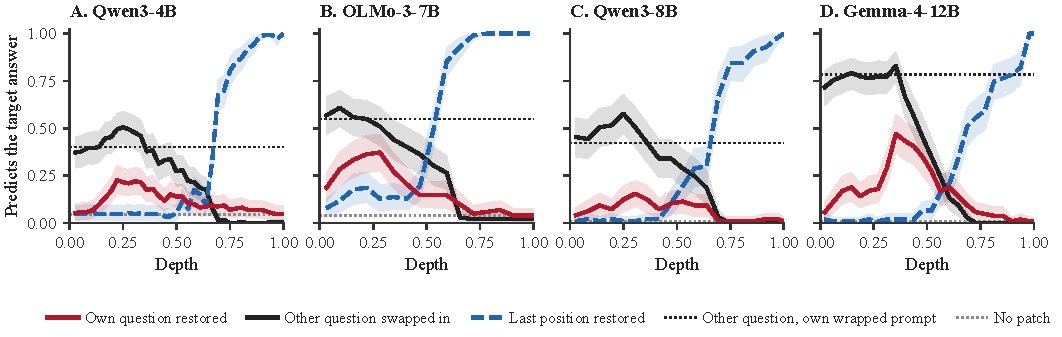
\includegraphics[width=\textwidth]{fig_swap.pdf}
\caption{\textbf{Patching failed wrapped prompts, by the depth of the patch.} Each solid or dashed line is the share of failed test prompts in which, after one patch at one layer, the model's most likely next token is the first token of the target answer. Red: the question's tokens are restored from the question's plain prompt; the target is its own answer. Black: the question's tokens are replaced by those of another question's plain prompt; the target is the other question's answer. Blue: the last position is restored from the plain prompt; the target is the question's own answer. Black dotted: how often the other question's answer is the most likely next token when that question is itself asked in the same wrapper. Grey dotted: the failed prompt without any patch. Bands are 95\% intervals.}
\label{fig:swap}
\end{figure*}

\subsection{Wrong answers replace weakly held ones}
\label{sec:confidence}

Which known answers are lost? We grouped known items by the probability the model gives the full answer in the plain prompt and counted what each wrapped prompt produced (Figure~\ref{fig:confidence}). The two kinds of failure behave differently.
\begin{itemize}
\item \emph{Wrong answers and ``not there'' claims hit weakly held answers.} Outside logs, among answers the model gives with probability 0.5--0.8, wrappers turn \OtherWrongLow{} into wrong answers and \OtherScopeLow{} into claims that the answer is not there. Above 0.999 these fall to \OtherWrongHigh{} and \OtherScopeHigh{}. A neutral sentence also loses more of the weakest answers (\NullLow{}, against at most \NullRest{} in the other groups), but far fewer than the wrappers.
\item \emph{Replies about the wrapper hit firm answers too.} Under logs, the share of replies that describe the log does not fall as the model grows more sure; it is \LogTaskLow{} for the weakest group and \LogTaskHigh{} for the firmest.
\end{itemize}
So a wrapper that changes the task overrides what the model knows, however firmly. The other failures mostly take answers the model holds weakly.

\subsection{The model reads the question; the answer is lost later}
\label{sec:where}

Where in the network is the answer lost? One possibility is that the wrapper changes how the model reads the question, so that the question's tokens no longer carry what the model needs. Another is that the question is read correctly, and the answer loses out later, at the position where the reply begins. Activation patching~\citep{vig2020causal,meng2022locating} can tell these apart. It reruns a failed wrapped prompt, replaces one internal state with its value from another run, and checks the result.

For each model we patched failed prompts in which the reply lost the answer and the answer's probability fell at least threefold; \NPairsTest{} of them are test items (Appendix~\ref{app:patching}). In each, at a single layer, we replaced one of three things:
\begin{enumerate}
\item \emph{Own question restored}: the states at the question's tokens, taken from the plain prompt of the same question.
\item \emph{Other question swapped in}: the states at the question's tokens, taken from the plain prompt of a different known question of the same kind and length in tokens, such as the capital of Sudan in place of the capital of Mongolia.
\item \emph{Last position restored}: the state at the last token of the prompt, from which the reply is produced, taken from the plain prompt of the same question.
\end{enumerate}
A state at a layer is the residual stream after that layer, and \emph{depth} is the fraction of the model's layers it has passed through. After each patch we checked whether the model's most likely next token is the first token of the target answer: the failed question's own answer for patches 1 and 3, and the other question's answer for patch 2. Without a patch this happens in \NoPatch{} of the failed prompts.

Two parts of Figure~\ref{fig:swap} hold by construction. At the first layer, swapping in another question's states is almost the same as asking that question inside the wrapper. At the last layer, restoring the last position copies the plain prompt's output. The evidence lies between these ends, and it gives three results that hold in every model.
\begin{itemize}
\item \emph{The swapped question is answered.} With another question's states in the first half of the network, the model gives the other question's answer in up to \SwapPeak{} of the prompts. The other question, asked inside the same wrapper, gets its answer as the most likely token in \DonorTopOne{} of cases. Up to about \HandoffDepth{} of the depth, the question's tokens decide which question the model answers, and the wrapper does not stop the model from answering it from memory.
\item \emph{Restoring the question's own states helps much less.} The failed question's own plain states bring its answer back in at most \RestorePeak{} of prompts at any single layer, and in \RestoreAll{} when restored at every layer at once. So the question is read about as well inside the wrapper as outside it, and its answer still loses. Logs are a partial exception: for the \NLogPairs{} log failures per model, restoring the question's states helps in up to \RestorePeakLog{} of prompts, so part of what logs damage is the reading of the question itself.
\item \emph{The answer is lost at the last position, after the question arrives there.} Restoring the last position does not help early in the network. It first brings the answer back in at least half of the prompts at \HandoffDepth{} of the depth, which is also where the swapped question stops having any effect. By then the question's content has moved from its own tokens to the last position, and the answer is lost after this move.
\end{itemize}
The model's probability of the full answer gives the same picture (Appendix~\ref{app:repair}).
